%% This skeleton file requires IEEEtran.cls version 1.6 or later.
%%
\documentclass[conference,letterpaper]{IEEEtran}
% If the IEEEtran.cls has not been installed into the LaTeX system files,
% manually specify the path to it:
%\documentclass[conference]{../sty/IEEEtran}
\IEEEoverridecommandlockouts
\overrideIEEEmargins

% some very useful LaTeX packages include:

\usepackage{cite}      % Written by Donald Arseneau
                        % V1.6 and later of IEEEtran pre-defines the format
                        % of the cite.sty package \cite{} output to follow
                        % that of IEEE. Loading the cite package will
                        % result in citation numbers being automatically
                        % sorted and properly "ranged". i.e.,
                        % [1], [9], [2], [7], [5], [6]
                        % (without using cite.sty)
                        % will become:
                        % [1], [2], [5]--[7], [9] (using cite.sty)
                        % cite.sty's \cite will automatically add leading
                        % space, if needed. Use cite.sty's noadjust option
                        % (cite.sty V3.8 and later) if you want to turn this
                        % off. cite.sty is already installed on most LaTeX
                        % systems. The latest version can be obtained at:
                        % http://www.ctan.org/tex-archive/macros/latex/contrib
%/supported/cite/

\usepackage[dvips]{graphicx}  % Written by David Carlisle and Sebastian Rahtz
                        % Required if you want graphics, photos, etc.
                        % graphicx.sty is already installed on most LaTeX
                        % systems. The latest version and documentation can
                        % be obtained at:
                        % http://www.ctan.org/tex-archive/macros/latex/required/graphics/
                        % Another good source of documentation is "Using
                        % Imported Graphics in LaTeX2e" by Keith Reckdahl
                        % which can be found as esplatex.ps and epslatex.pdf
                        % at: http://www.ctan.org/tex-archive/info/

\usepackage{amsmath}   % From the American Mathematical Society
                        % A popular package that provides many helpful commands
                        % for dealing with mathematics. Note that the AMSmath
                        % package sets \interdisplaylinepenalty to 10000 thus
                        % preventing page breaks from occurring within multiline
                        % equations. Use:
\usepackage{amssymb}

\usepackage{multirow}
\usepackage[left=0.71in,top=0.94in,right=0.71in,bottom=1.18in]{geometry}
\setlength{\columnsep}{0.24in}
% correct bad hyphenation here
%\hyphenation{op-tical net-works semi-conduc-tor IEEEtran}

%New theorems
\newtheorem{fact}{Proposition}
\newtheorem{definition}{Definition}
%New commands
\newcommand{\q}{\mathbf q}
\newcommand{\dq}{\dot {\mathbf q}}
\newcommand{\deltauhand}{\Delta \mathbf {u}_{hand}}
\newcommand{\deltaqarm}{\Delta \mathbf {q}_{arm}}
\newcommand{\qarm}{\mathbf q_{arm}}
\newcommand{\jacobian}{\mathbf J}
\newcommand{\uhand}{\mathbf{u}_{hand}}
\newcommand{\utarget}{\mathbf{u}_{target}}
\newcommand{\xhand}{\mathbf{x}_{hand}}
\newcommand{\qhead}{\mathbf{q}_{head}}
\newcommand{\xtarget}{\mathbf{x}_{target}}

\begin{document}
% paper title
\title{\huge Learning precise 3D reaching in a humanoid robot}

% author names and affiliations
\author{\authorblockN{Lorenzo Natale}
\authorblockA{
\textit{Italian Institute of Technology}\\
\textit{Via Morego 30, Genova, ITALY}\\
\textit{lorenzo.natale@iit.it}\\}%
\and
\authorblockN{Francesco Nori}
\authorblockA{
\textit{Italian Institute of Technology}\\
\textit{Via Morego 30, Genova, ITALY}\\
\textit{francesco.nori@iit.it}\\}
\and
\authorblockN{Giorgio Metta}
\authorblockA{
\textit{Italian Institute of Technology}\\
\textit{Via Morego 30, Genova, ITALY}\\
\textit{giorgio.metta@iit.it}\\}
}%

% make the title area
\maketitle
\begin{abstract}
In this paper we discuss the implementation of a precise reaching controller 
on an upper torso humanoid robot. The proposed solution is based 
on a learning strategy which does not rely on \emph{a priori} models of either
the arm or head kinematics. After learning the robot can reach for visually 
identified objects, in the 3-dimensional space. Reaching integrates together 
an open loop and a closed loop strategy; the open loop allows ballistic 
movements, while the closed loop performs precise positioning of the hand in 
the visual space. Differently from other approaches we handle the critical 
case of redundancy in the head and arm. 
\end{abstract}

% key words
\begin{keywords}
Visual servoing, reaching, learning, development, humanoid robotics.
\end{keywords}
%
\section{Introduction}
Put here the introduction.
%

\section{Previous Works}

[-] locating an observed object with respect to the robot requires the following data:
		[*] robot forward kinematic (analytical or estimated)
		[*] cameras calibration (self or grid calibration)
		[*] hand-eye calibration 
		
[-] visual servoing requires:
		[*] the manipulator jacobian dx_hand = J(q_arm) dq_arm
		[*] the interaction matrix ds = L(q_head, q_arm) dx_hand
\subsection{Robotic setup}
\textit{James} is an \textit{upper-torso humanoid robot} with the size of an 
about ten years old boy, a total weight of about 8 kilograms and 22 degrees 
of freedom (DOF) \cite{JHRAUW06-12}. James consists of a head on a special 
neck , a left arm with a peculiar shoulder and the torso.

\begin{figure}
\centering
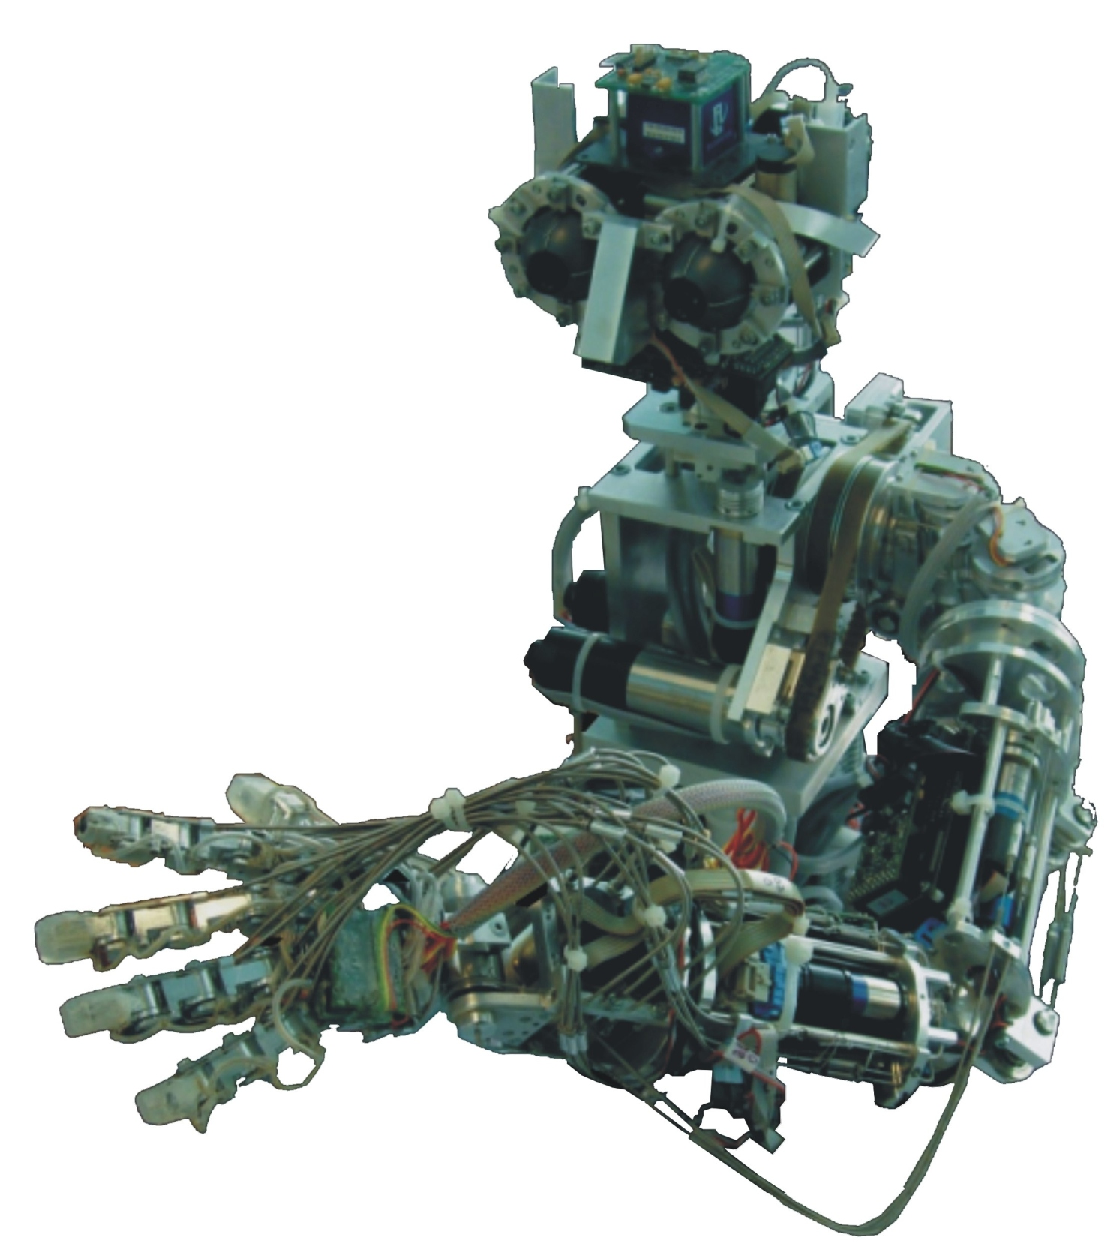
\includegraphics[width=2in]{imgs/james.ps}
\caption{James}
\label{figJames}
\end{figure}

\section{Gaze control}
\label{Sec:gazecontrol}

In this section we describe how we control the gaze of the robot to
fixate a visual target.
%
\begin{figure}[tbp]
\centering
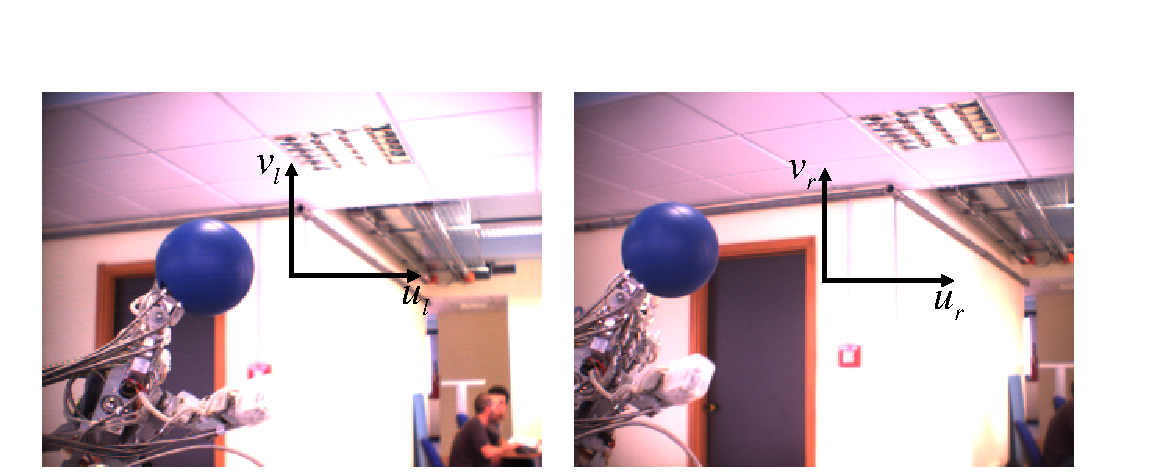
\includegraphics[width=8cm]{Figure/hand.eps}
%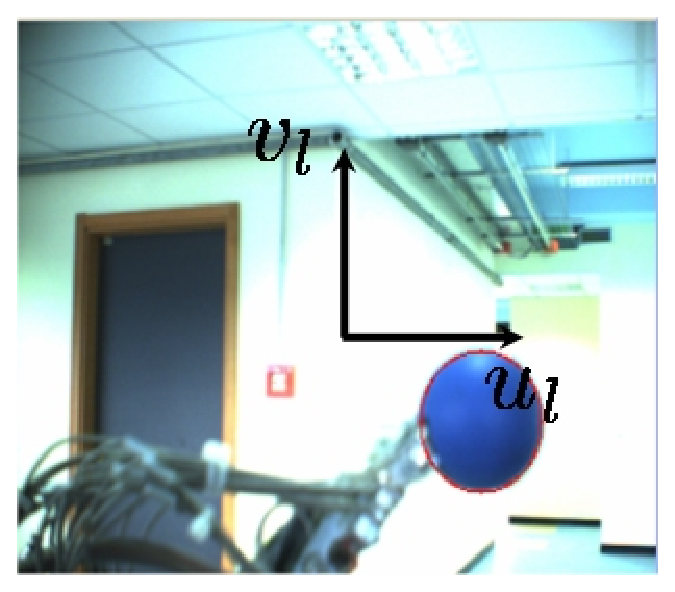
\includegraphics[width=25mm]{Figure/LeftImage.eps} \hspace{1cm}
%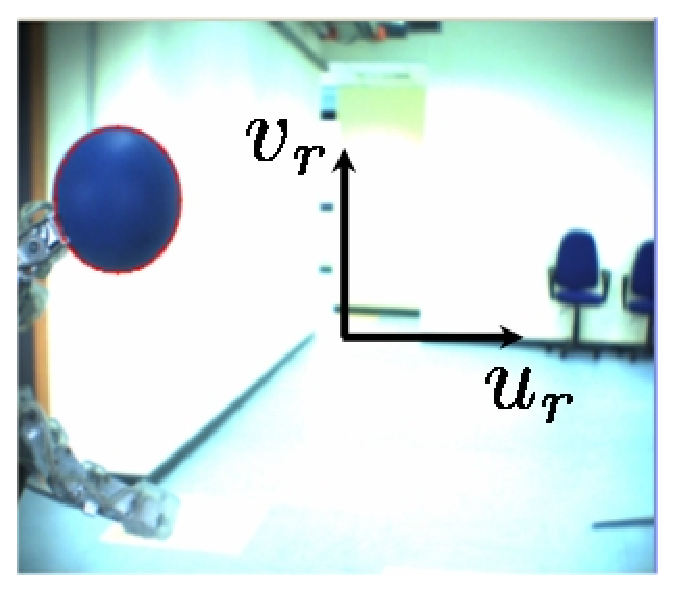
\includegraphics[width=25mm]{Figure/RightImage.eps}
\caption{Two typical images taken from the cameras mounted on the 
eyes of the robot (resolution 320$\times$240).
The coordinates of the target (the blue ball) on the image planes
will be denoted $u_l$, $v_l$, and $u_r$, $v_r$ (respectively left 
and right cameras).}
\label{Fig:ImagePlane}
\end{figure}
% 
The crucial aspect in this case concerns the redundancy of the 
head. Let $u_r$ and $v_r$ be the coordinates of the target on the 
right image plane. Similarly, let $u_l$ and $v_l$ be the coordinates 
of the target on the 
left image plane (see Figure \ref{Fig:ImagePlane}). The values of $u_r$, 
$v_r$, $u_l$, $v_l$ are the output of a visual module which detects the
target in the image planes. Directing gaze 
toward the target 
consists of moving the neck and the eyes so as to obtain 
$u_r=0$, $v_r=0$, $u_l=0$, $v_l=0$. 
Let us define the vector 
$\tilde {\mathbf u}_{target}= \begin{bmatrix} u_r & v_r & u_l & v_l 
\end{bmatrix}^\top \in \mathbb R^4$ corresponding to the 
target location in the image planes. Under reasonable 
assumptions, we do not need to impose simultaneously 
the four conditions $u_r=0$, $v_r=0$, $u_l=0$, $v_l=0$.  Our control task 
can be redefined as the problem of controlling 
$\utarget = \begin{bmatrix} u_r & u_l & v_l \end{bmatrix}^\top \in \mathbb R^3$ 
to zero. Clearly, the task specification does not constrain all the head 
degrees of freedom (we are imposing $3$ constraints but we 
have $6$ free variables available). 
We solve this ``redundancy problem'' by using two controllers for the 
eyes and the neck. The former controls 
the eyes version and common tilt to track the object, while the latter
controls neck yaw and pitch to maintain the eyes ``centered'' within 
the neck. Mathematically the above strategy can be implemented 
as follows:
%
\begin{eqnarray} \label{Eq:HeadEyeControl}
\left\{\begin{matrix}
\dot {\alpha_v^c} &=&   K_p (u_l + u_r)\\
\dot {\theta_y} &=&   K_y \alpha_v^c 
\end{matrix}
\right.,\quad
\left\{ \begin{matrix}
\dot {\alpha_t^c} &=&   K_t (v_l + v_r)\\
\dot {\theta_p} &=&   K_r \alpha_t^c
\end{matrix} \right.,
\end{eqnarray}
%
where $\alpha_v^c$ and $\alpha_t^c$ are the eyes tilt and common version and 
where $\theta_y$ and $\theta_p$ are the yaw and pitch movement of the neck. 
In the proposed control scheme, the vergence degree of freedom $\alpha_v^d$, 
which corresponds to the distance of the target does not influence 
the neck position and is therefore controlled separately from the neck:
\begin{eqnarray} 
\dot {\alpha_v^d} &=&   K_p (u_l - u_r).
\end{eqnarray}
Finally, the neck roll degree of freedom $\theta_r$ is maintained fixed, 
i.e. $\theta_r^d=0$.

The proposed control strategy allows us to asymptotically fixate the target 
($u_l \rightarrow 0$, $v_l \rightarrow 0$, $u_r \rightarrow 0$ which 
implies $v_r \rightarrow 0$) while, at least within the mechanical limits 
of the head, also guaranteeing a straight gaze 
($\alpha_v^c \rightarrow 0$, $\alpha_t^c \rightarrow 0$). 
%Moreover, by choosing a suitable value for the gains 
%$K_p$, $K_y$, $K_t$ and $K_r$ it is possible to achieve an asymptotic 
%behavior with the eyes moving rapidly on the target and the neck following 
%the eye movement with a slower movement.

\section{Reaching}
\label{sec:reaching}

In this section, we describe the two approaches we followed to solve
the reaching task on our robot. The first method 
uses the forward mapping between the arm joint space and the three 
dimensional position of the hand represented in the head reference 
frame. The second method uses a visual servoing technique to control the 
speed of the arm to minimize the position of the hand in the 
image plane with respect to a desired target (the fixated object).

\subsection{Open Loop Reaching}
%
Suppose that the robot is tracking a target as described 
in Section \ref{Sec:gazecontrol}. In the assumption of perfect 
tracking (the visual error is zero), the three dimensional spatial position 
of the target with respect to the robot, denoted $\tilde {\mathbf x}_{target} 
\in \mathbb R^3$, 
is a function of the head configuration $\mathbf q_{head} =
\begin{bmatrix} \theta_y & \theta_p & \theta_r & \alpha_v^d & \alpha_v^c & \alpha_t^c \end{bmatrix}^\top \in \mathbb R^6$.
However, the representation of the target position, 
$\tilde {\mathbf x}_{target}$, in terms of the full head configuration, 
$\mathbf q_{head}$, is redundant.
Specifically, the same target position can be represented by different 
head configurations. To obtain a one to one mapping between the target 
position and the head configuration we have to analyze the 
gaze controller. The latter maintains $\theta_r$ stationary 
($\theta_r^d = 0$) and poses additional constraints on the head joints. 
In particular the controller minimizes 
$\alpha_t^c$ and $\alpha^c_v$ (see equation 
(\ref{Eq:HeadEyeControl})) so that they converge to zero 
($\alpha_t^c \rightarrow 0$ and 
$\alpha_v^c \rightarrow 0$). Ideally, after fixation is achieved, we have 
$\mathbf {q}_{head}=
\begin{bmatrix} \theta_y & \theta_p & 0 & \alpha_v^d & 0 & 0 \end{bmatrix}^\top \in \mathbb R^6.
$
%
Since there exists a one to one mapping between the three dimensional 
position of the target 
$\tilde {\mathbf x}_{target}$ and the three non-zero variables 
$\theta_y$, $\theta_p$ and $\alpha_v^d$, we can define $
\mathbf x_{target}=
\begin{bmatrix} \theta_y & \theta_p & \alpha_v^d\end{bmatrix}^\top \in \mathbb R^3.
$
%
This new variable $\mathbf x_{target} \in \mathbb R^3$ uniquely codes the 
spatial position of the target in a way that resembles a three dimensional 
polar representation. In particular $\theta_y$ and $\theta_p$ code  
\emph{azimuth} and \emph{elevation}, while \emph{distance} is 
substituted with $\alpha_v$ (the \emph{vergence} angle). 

If the robot tracks the hand, the same subset of the head joint space 
can be used to code the spatial location of the hand: $
\xhand=
\begin{bmatrix} \theta_y & \theta_p & \alpha_v^d\end{bmatrix}^\top \in \mathbb R^3.
$
%
Under these assumptions, the \emph{forward mapping} 
$f_{arm}$
relates the arm configuration $\qarm$ with the position of the hand 
$\xhand$:
%
\begin{equation} 
\label{Eq:forward}
\mathbf x_{hand}=f_{arm}(\mathbf q_{arm}), \qquad f_{arm} : \mathbb R^4 \longrightarrow \mathbb R^3.\end{equation}
%
In the next section we show how a neural network could be trained to 
approximate $f_{arm}$.% (Eq. \ref{Eq:forward}).

Suppose now that the robot is fixating a target and that we want to control 
the robot to reach for it. Formally the problem can be formulated 
as determining the value of $\qarm$ which solves the 
following optimization problem:
%
\begin{equation} 
\label{Eq:reaching1}
  \displaystyle\min_{\qarm}
  \left\|\mathbf x_{hand} - \mathbf x_{target}\right\|^2,
\end{equation}
%
where $\mathbf x_{target}$ is measured from the encoders of the head, while 
$\mathbf x_{hand}$ is computed from $\qarm$ through Eq. (\ref{Eq:forward}).
Given the redundancy of the arm kinematics this minimization has infinite 
solutions. We constrained the problem by 
forcing one of the joints, for example joint number 2 (one of the shoulder 
joints), to remain as close as possible to a predefined value $q_{20}$:
%
\begin{equation} 
\label{Eq:reaching2}
  \displaystyle\min_{\qarm}
  \left[
  \left\|\mathbf x_{hand} - \mathbf x_{target}\right\|^2 + \left(q_{arm,2}-q_{20}\right)^2
  \right].
\end{equation}

The optimization of (\ref{Eq:reaching2}) can be performed numerically using 
various algorithms. In our implementation, we used 
the downhill simplex method \cite{ne:Computer:65}. 
% as implemented in \cite{mo:Press:90}.

\subsection{Learning the open loop reaching}
\label{sec:learning-open-loop}
%
To learn the forward map of Eq. (\ref{Eq:forward}) we programmed 
the robot to perform random movements with the arm (chosen to uniformly sample 
a predefined region in the robot workspace). During this ``exploratory'' 
phase the robot tracked the hand, and collected samples of the form: $
%
\left(\begin{array}{cc}
  \qarm^i , \xhand^i\end{array}\right)_{i = 0,1\dots}$.
%
 A neural network was then trained to learn the relation:
%
\begin{equation}
  \label{eq:openloop}
  \xhand=\hat{f}_{arm}\left(\qarm \right),
\end{equation}
%
which approximates Eq. (\ref{Eq:forward}).

In the experiment reported in this paper we collected a data set of 
about 2890 samples that we divided in a training set ($N_{train}=2168$
 samples) and 
a test set ($N_{test}=725$ samples). The neural network we employed was the 
Receptive Field Weighted Regression model proposed 
by \cite{schaal98Constructive}. This network implements an online learning
method, meaning that a learning step is performed every time a new 
sample is presented to the network. All samples in the training set were shown
to the network in a random order. After each training step the 
performance of the network was validated on the whole test set, by computing
the Mean Squared Error (\emph{MSE}) between each sample in the test set, 
%$$\xhand^i$,
and the corresponding network output.
%$\mathbf{\hat{x}}_{hand}^i$:
%
%\begin{equation}
%\emph{MSE}=\frac{1}{N_{test}}\sum_{i=0}^{N_{test}-1}\|\xhand^i- \hat{\mathbf{x}}_{hand}^i\|^2
%\end{equation}
%

The plot in figure \ref{Fig:learningerrors}
shows the trend of the error on the test set during learning. At the end of
the training the network reached the performance of $\emph{MSE}=5.7~deg^2$ 
(with $\emph{STD}=10.4~deg^2$).

In the experiment reported in this paper the network was trained offline. 
This was done to simplify the analysis of the results and to perform 
cross-validation on a predefined test set. However, the learning algorithm 
we used is purely incremental (each sample was shown to the network only 
once and immediately 
discarded), so in this regard it would be straightforward to convert the 
same approach to an online implementation.

\subsection{Closed Loop Reaching} \label{Eq:ClosedLoop}
%
If the robot could visually measure the distance
between the hand and the target, reaching could also be solved
visually by implementing a closed control loop. This 
consists in performing a preliminary (open loop) reaching movement and 
then refining the action by visually correcting any residual error. 

We know that the Jacobian matrix relates arm velocities 
$\dot {\mathbf q}_{arm}$
with hand velocities in the image plane $\dot {\mathbf u}_{hand} = \left[ 
\begin{array}{ccc}
  \dot u_r & \dot u_l & \dot v_{l}
\end{array} \right]^\top$:
\begin{equation} 
  \dot {\mathbf u}_{hand}=
  \tilde{\mathbf J}\left(\mathbf q_{arm}, \mathbf q_{head}\right)
  \dot {\mathbf q}_{arm},
\end{equation}
where $\tilde{\jacobian} \in \mathbb R^{3 \times 4}$ depends on 
both the configuration of the arm and the head. In practice, assuming 
sufficiently small arm movements $\deltaqarm$, we can use the following 
approximation:
%
\begin{equation} 
\label{eq:jacobian1}
  \deltauhand=
  \tilde{\mathbf J}\left(\mathbf q_{arm}, \mathbf q_{head}\right)
  \deltaqarm,
\end{equation}
where $\deltauhand$%= $[ \Delta u_r$, $\Delta u_l$, $\Delta v_{l}]^\top$ 
is the image plane displacement resulting from the arm movement $\deltaqarm$. 
Due to the additional constraints posed by the head tracker, we showed
that only a subset of $\qhead$, $\xtarget$, is 
sufficient to uniquely identify the position of the head, so we 
can rewrite equation (\ref{eq:jacobian1}) as:
%
\begin{equation}
\label{eq:jacobian2}
  \deltauhand=
  \tilde{\jacobian}\left(\qarm, \xtarget\right)
  \deltaqarm, \qquad \tilde{\jacobian} \in \mathbb R^{3 \times 4}.
\end{equation}
%

Moreover, after the preliminary open loop reaching movement, we know
that $\xtarget = f_{arm}(\qarm)$ so that  Eq.
(\ref{eq:jacobian2}) can be further simplified to:
%
\begin{equation} 
\label{eq:jacobian3}
  \deltauhand=
  \jacobian \left(\qarm\right)
  \deltaqarm,\qquad \jacobian \in \mathbb R^{3\times4}
\end{equation}
%
where $\jacobian$ depends only on the arm joint configuration $\qarm$. 

Suppose now that the robot has to reach for an object, whose visual 
position is 
represented by $\utarget$. To solve this problem 
the controller of the arm needs to compute the arm command which minimizes 
the error $e=\left\|\uhand-\utarget\right\|^2$.
%
%
When the head tracker has achieved convergence on the object, 
$\utarget \approx 0 $ and $e$ $\approx \left\|\uhand\right\|^2$.
Due to the redundancy of the arm, the minimization of $e$ can have
infinite solutions. Among them, the minimum norm solution corresponds
to the minimum joint speeds, that is:
%
\begin{equation}
\mathbf{\dot q}_{arm}=-k \cdot \jacobian^\# \uhand, 
\qquad \jacobian^\# \in \mathbb R^{4 \times 3},
\end{equation}
%
where $\jacobian^\#$ is the Moore-Penrose pseudo-inverse of $\jacobian$.
In practice $\xtarget = f_{arm}(\qarm)$ is estimated through 
Eq. \ref{eq:openloop}, so only an approximated value 
$\hat{\jacobian}^\#$ will be available. Convergence is guaranteed 
if $\hat{\jacobian}^\#\cdot\jacobian>0$ \cite{samson91robot}.


%The next section describes a procedure by which the robot can 
%autonomously acquire $\jacobian$ and $\jacobian^\#$.

\subsection{Learning the Arm Jacobian}
\begin{figure}
  % Requires \usepackage{graphicx}
  \begin{center}
	\begin{tabular}{ccc}
	  \parbox{40mm}{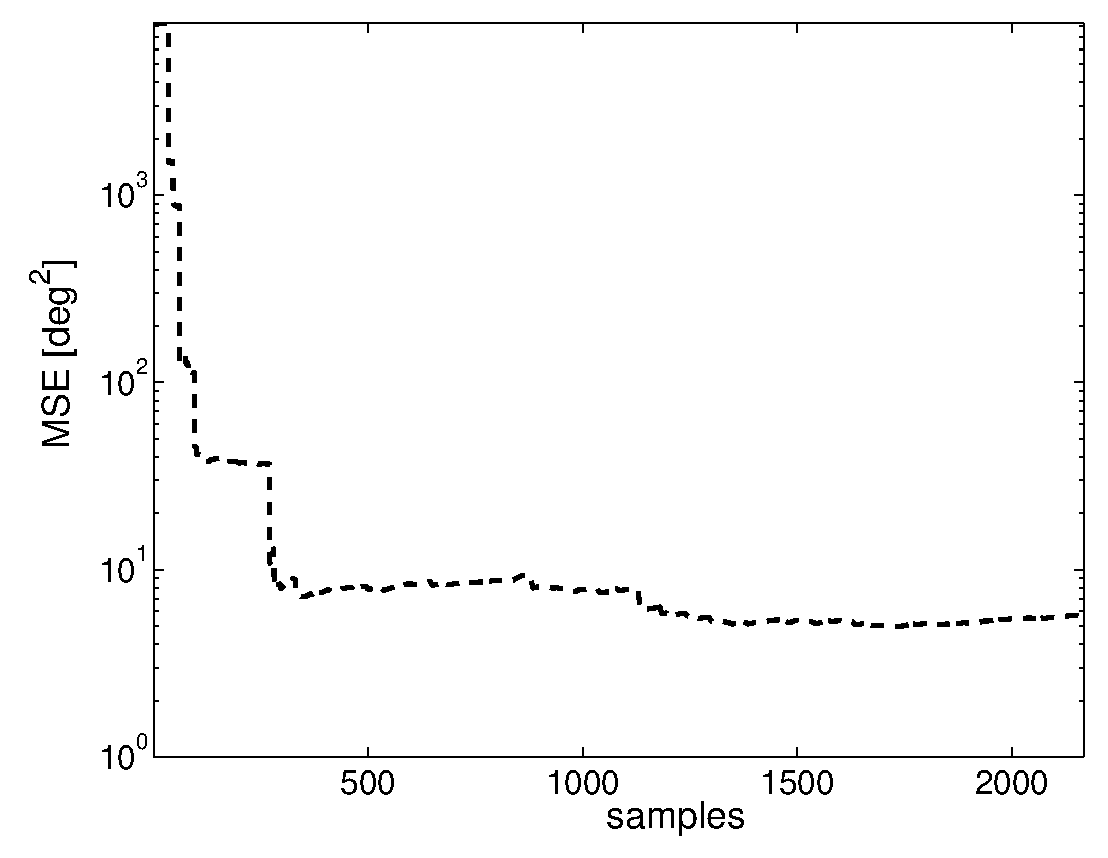
\includegraphics[width=40mm]{./Figure/reachingError1.eps}}  & \hspace{.1cm} &
	  \parbox{35mm}{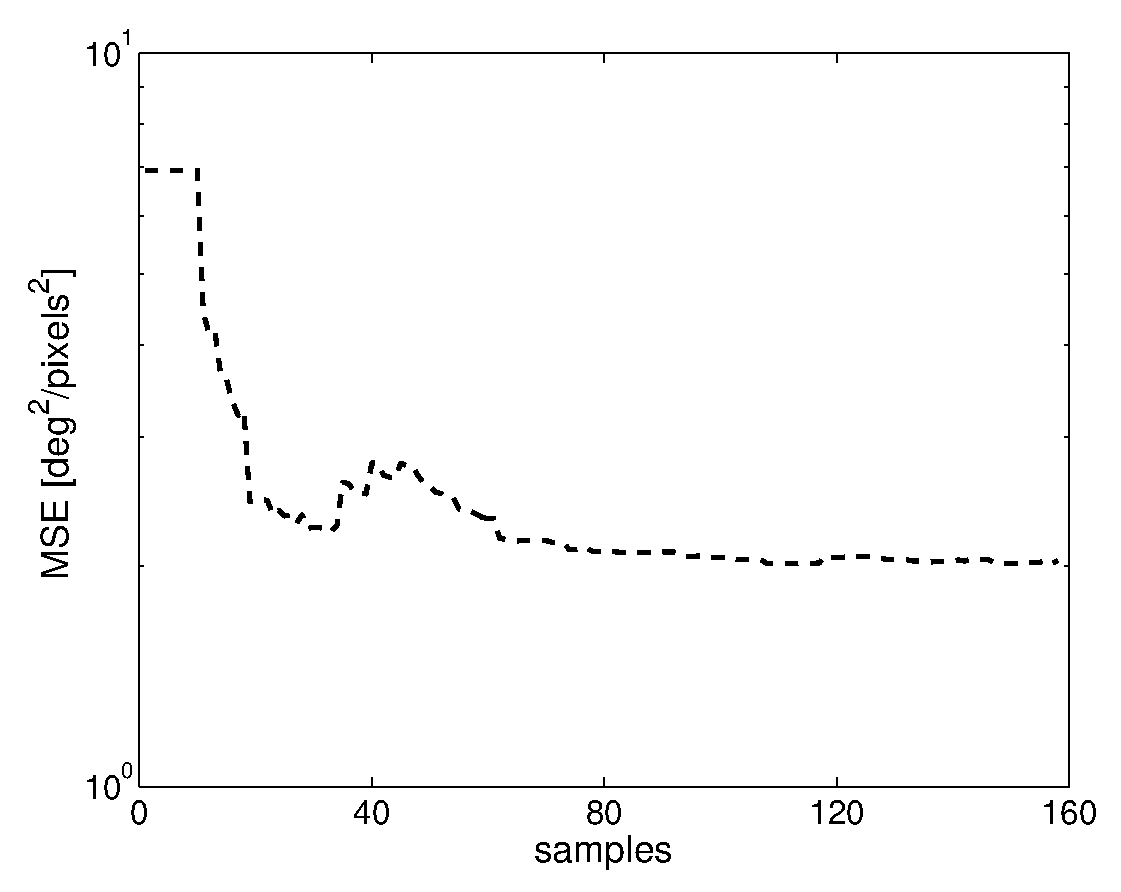
\includegraphics[width=40mm]{./Figure/jacobian-error.eps}}
  \end{tabular}
\end{center}
\caption{Left: learning of the arm forward function. Right: learning the 
arm jacobian. The plots represent the \emph{MSE} on 
the test set during learning. See text for more details}\label{Fig:learningerrors}
\end{figure}
%
%
%In the previous section we used the Jacobian of the manipulator
%$\jacobian$ (actually its pseudo-inverse $\jacobian^\#$) to 
%control the arm to reach for a visually identified object. In 
%this section we describe a procedure by which the robot can 
%autonomously acquire $\jacobian$ and $\jacobian^\#$.
%
As described in Section \ref{sec:learning-open-loop}, the robot 
moves the arm randomly, while maintaining gaze on the hand. At 
the end of each movement $j$ the arm is in a configuration 
$\qarm^j$,  while the eyes are fixating the hand 
($\uhand \approx 0$). %with a straight gaze
%(the head tracker has reached convergence).%
Each arm configuration corresponds to a different value of 
$\jacobian_j=\jacobian\left(\qarm^j\right)$. 
Now the robot inhibits the head tracker and performs a sequence $m$
of small arm movements $\deltaqarm^k$ which perturb $\uhand$ of small 
amounts $\deltauhand^k$:$
  \left(\begin{array}{cc}
    \deltauhand^k , 
	\deltaqarm^k \end{array}
  \right)_{k = 0,1\dots,m}
$. All $m$ perturbations $\deltauhand^k$ and 
$\deltaqarm^k$ are linearly related through $\jacobian_i$ 
as described in Eq. (\ref{eq:jacobian2}). From these $m$ 
observations we can derive a least squares estimation of $\jacobian_j$ from 
which, in turn, we can compute the pseudo-inverse $\jacobian_j^\#$. 

Re-iterating this procedure leads to the collection of a series of examples:
$\left(\begin{array}{cc}
\qarm^j , \jacobian_j^\# \end{array}\right)_{j = 0,1\dots}$.
An approximation $\hat{\jacobian}^\#$ of $\jacobian^\#$ is finally
obtained by training a neural network:
%
\begin{equation}
\mathbf{g}\left(\qarm\right), \qquad g : \mathbb R^4 \longrightarrow \mathbb R^{12},
\end{equation}
%
whose output components are the coefficients of 
$\hat{\jacobian}^\# \in \mathbb R^{4 \times 3}$.

We report here the result of a learning session. The robot explored 210 
different arm positions $\qarm^j$ randomly distributed within a region of 
the workspace. In each of these positions the robot executed $m=10$ 
perturbations $\deltaqarm^k$ and estimated an example $\jacobian^\#_j$ for 
the neural network. Overall we collected 210 samples for $\jacobian^\#$. 
We trained the neural network on a subset of $N_{train}=158$ elements 
(training set); each 
sample was shown to the network only once and then discarded. Following each 
training step, we evaluated the performance of the network by computing 
\emph{MSE} on the remaining $N_{test}=52$ elements 
(test set). At the 
end of the training the error on the test set was 
$\emph{MSE}=2~\frac{pixels^2}{deg^2}$ 
($\emph{STD}=7.1~\frac{pixels^2}{deg^2}$). Figure \ref{Fig:learningerrors} reports the plot of the error during learning.
%

\section{Results}
\label{sec:results}

In this section we report the results of the experiments we carried out
to quantify the performance of the reaching movements. Following the proposed strategy, 
in order to reach for the 
target we first need to fixate it, i.e. $\utarget = 0$. Using the available sensor (i.e. vision) the best we can do to precisely reach the target is moving the hand to the fixation point, i.e. $
{\uhand} \longrightarrow 0$. Clearly, the image plane distance $\| \uhand - \utarget \|$ can be used as a rough estimate of the reaching precision, i.e. of the Cartesian distance between the target to be reached and the position of the hand. Specifically, assuming infinite resolution of the camera sensor, if $\| \uhand - \utarget\| = 0$ then the hand has exactly reached the target.

\subsection{Open Loop}
The first attempt to reach the target consists in using the learned forward model 
(\ref{Eq:forward}) and the strategy (\ref{Eq:reaching2})
to choose the arm configuration $\q_{arm}$ which brings the hand to the center 
of the image planes. Clearly, if the forward 
kinematic function (\ref{Eq:forward}) were perfectly represented and if the target were reachable, then we would have 
$\mathbf x_{hand} =  \mathbf x_{target}$, which implies that the target-hand Cartesian distance 
 is zero (see Section \ref{sec:reaching} for details). Therefore, in this ideal case, the open loop 
 strategy already results in $\| \uhand - \utarget \| = 0$. In practice, the model 
 (\ref{Eq:forward}) cannot exactly represent the system's kinematic\footnote{Part of the representational 
 errors are related to the representation of the kinematic function, in this case the
 so called Receptive Field Weighted Regression model. Part are due to the mechanical plays and backlash of the
 mechanical structure.}. Therefore, even tough we can find $\q_{arm}$ such that $\mathbf x_{hand}=
 \hat f_{arm}(\mathbf q_{arm})$ it is not guaranteed that after the movement execution 
 $\| \uhand - \utarget \| = 0$. Figure \ref{Fig:ImagePlaneOpenLoopErrors}
 shows the image plane errors after the execution of the open loop movement. The plot has been obtained
 by fixating a target and performing a series of open loop movements. Each open loop
 movement was different because (\ref{Eq:reaching2}) was solved 
 by choosing a different value $q_{20}$. 


\begin{figure}
  % Requires \usepackage{graphicx}
  \begin{center}
	\begin{tabular}{ccc}
	  \parbox{30mm}{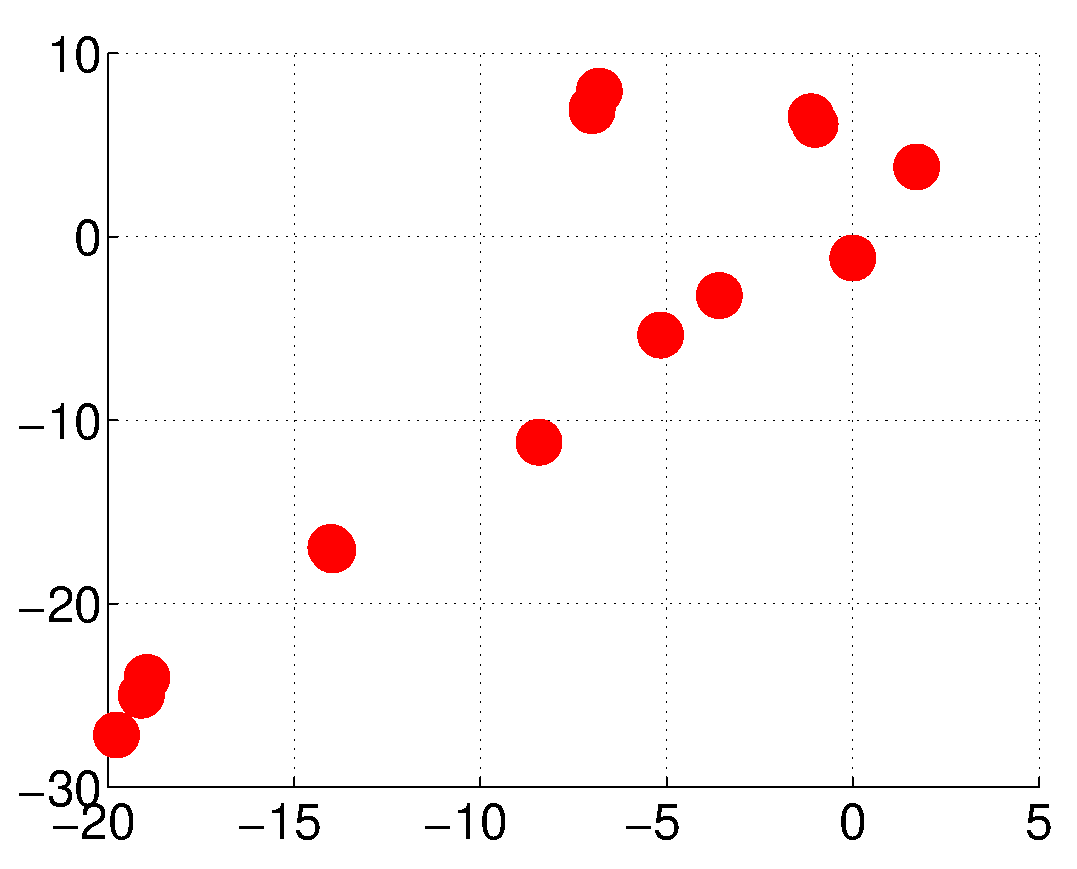
\includegraphics[width=30mm]{Figure/LeftEyeOpenLoop.eps}}  & \hspace{0.1cm} &
	  \parbox{30mm}{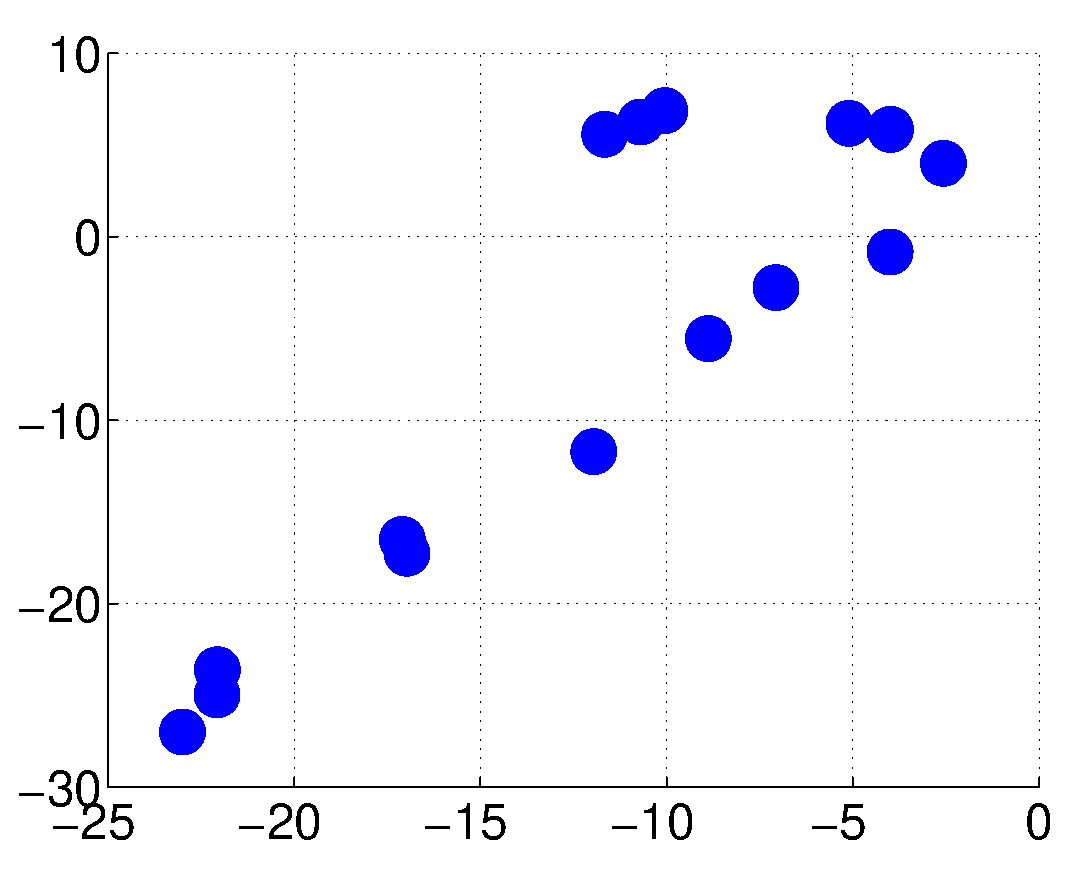
\includegraphics[width=30mm]{Figure/RightEyeOpenLoop.eps}}
	  \\
	  \parbox{30mm}{\centering Left eye } & \hspace{0.1cm} & \parbox{30mm}{\centering Right eye }
	  %	  \end{t\\
	  %	Top view & & Lateral view
  \end{tabular}
\end{center}
\caption{Open loop image plane errors $\uhand$ for different
choices of the redundant variable $q_{20}$. On the horizontal axis 
$u_r$ and $u_l$; vertical axis $v_r$ and $v_l$ (always in pixels).
The hand position in the image plane is represented 
by the small circles.  Each circle corresponds to a different open loop movement, i.e. a different value of $q_{20}$.
}\label{Fig:ImagePlaneOpenLoopErrors}
 \end{figure}

\subsection{Closed Loop}

The residual image plane errors 
due to imperfections in the forward kinematic model can be reduced by a visual closed loop
control strategy (\ref{Eq:ClosedLoopStrategy}), started immediately after the open loop phase. Relatively weak conditions on the learned 
Jacobian \cite{Samson91robot} guarantee the convergence of the image plane errors $\uhand$ to zero, and therefore
the convergence of the hand $\xhand$ on the target $\xtarget$. Figures
\ref{Fig:ImagePlaneClosedLoopErrors}, %\ref{Fig:TimeResponseClosedLoopErrors}, 
\ref{Fig:TimeResponseOpenClosedLoopErrors} and \ref{Fig:TimeResponseOpenClosedLoop}  
show how the hand is actually driven to the 
exact image center in both the image planes. The closed loop controller 
improves the accuracy of the reaching movement, but at the cost of a slower 
execution speed (see Figure \ref{Fig:TimeResponseOpenClosedLoop}); faster
executions couldn't be obtained by increasing the control loop gains, due to
the frame rate (thirty milliseconds) and the delays in the visual processing (hand localization and tracking).
Finally, it is important to notice 
the quasi-linearity of the path followed by the hand 
(see Figure \ref{Fig:ImagePlaneClosedLoopErrors}). This linearity denotes 
a good accuracy of the learned Jacobian.

\begin{figure}[th!]
  % Requires \usepackage{graphicx}
  \begin{center}
	\begin{tabular}{ccc}
	  \parbox{30mm}{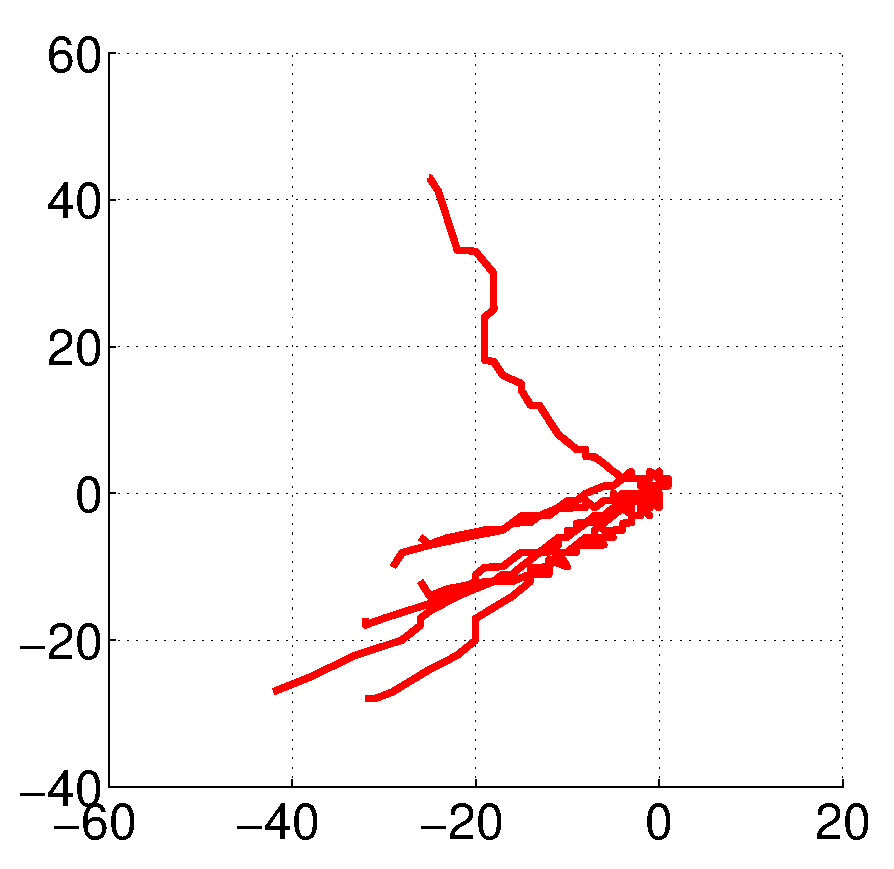
\includegraphics[width=30mm]{Figure/LeftEyeClosedLoop.eps}}  & \hspace{.1cm} &
	  \parbox{30mm}{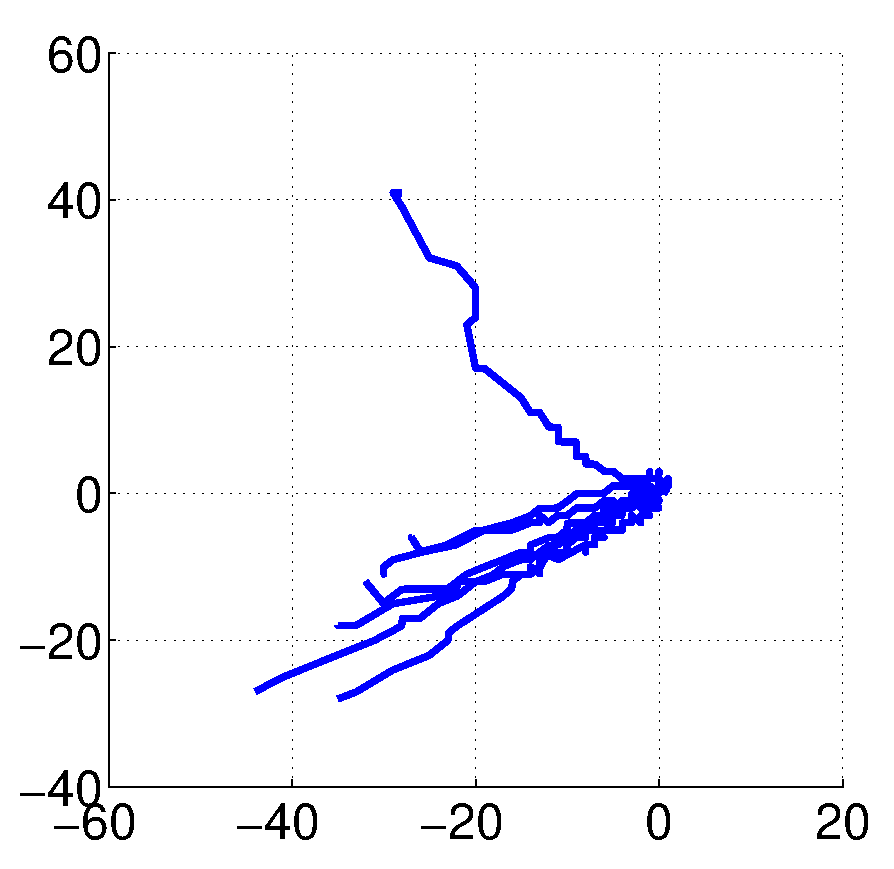
\includegraphics[width=30mm]{Figure/RightEyeClosedLoop.eps}}
	  \\
	  \parbox{30mm}{\centering Left eye } & \hspace{0.1cm} & \parbox{30mm}{\centering Right eye }
	  %	  \end{t\\
	  %	Top view & & Lateral view
  \end{tabular}
\end{center}
\caption{Traces of different closed loop control actions. Each trace correspond to a different Cartesian position of the target to be reached (which 
is always at the center of the image planes). All the traces end up in the image center thus indicating that the visual errors are completely eliminated by the closed loop controller.}\label{Fig:ImagePlaneClosedLoopErrors}
  \end{figure}

%\begin{figure}
%  % Requires \usepackage{graphicx}
%  \begin{center}
%	\begin{tabular}{ccc}
%	  \parbox{30mm}{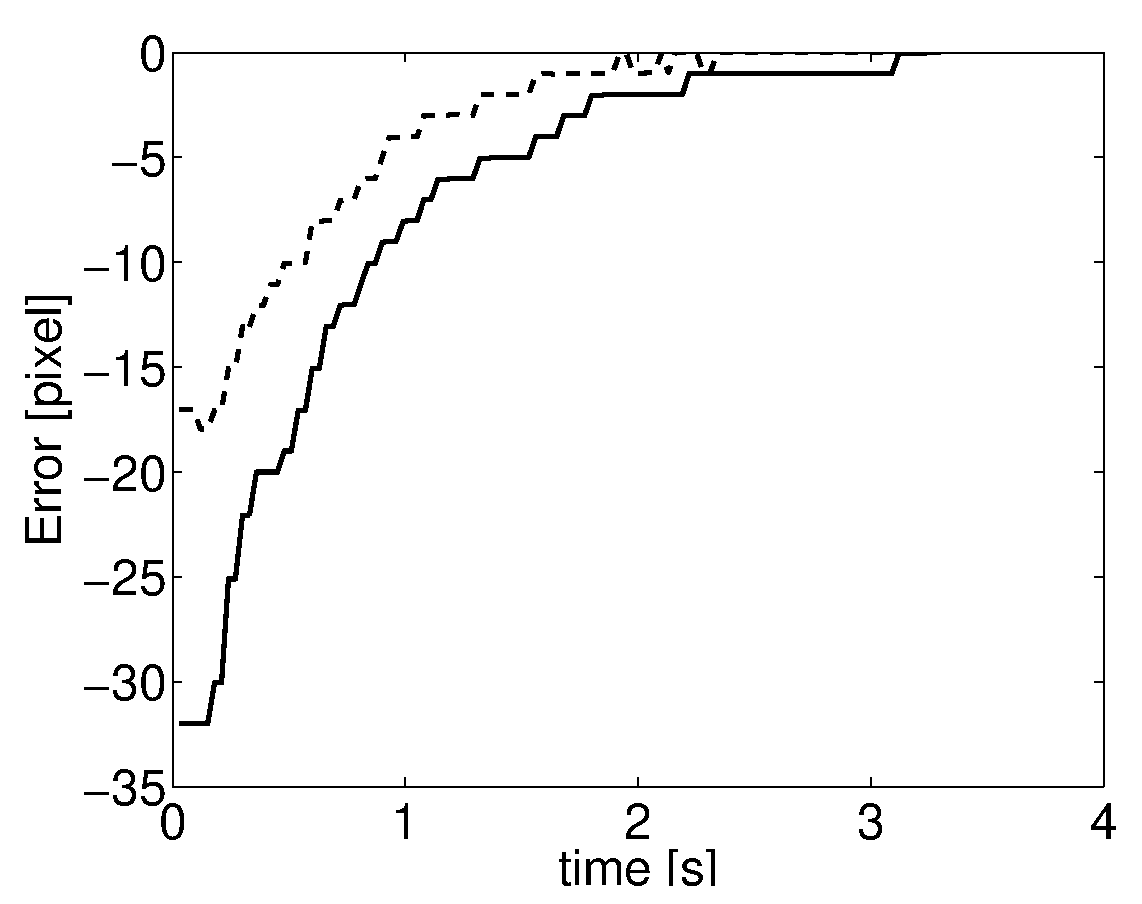
\includegraphics[width=30mm]{Figure/TimeReponseLeftClosedLoop.eps}}  & \hspace{.1cm} &
%	  \parbox{30mm}{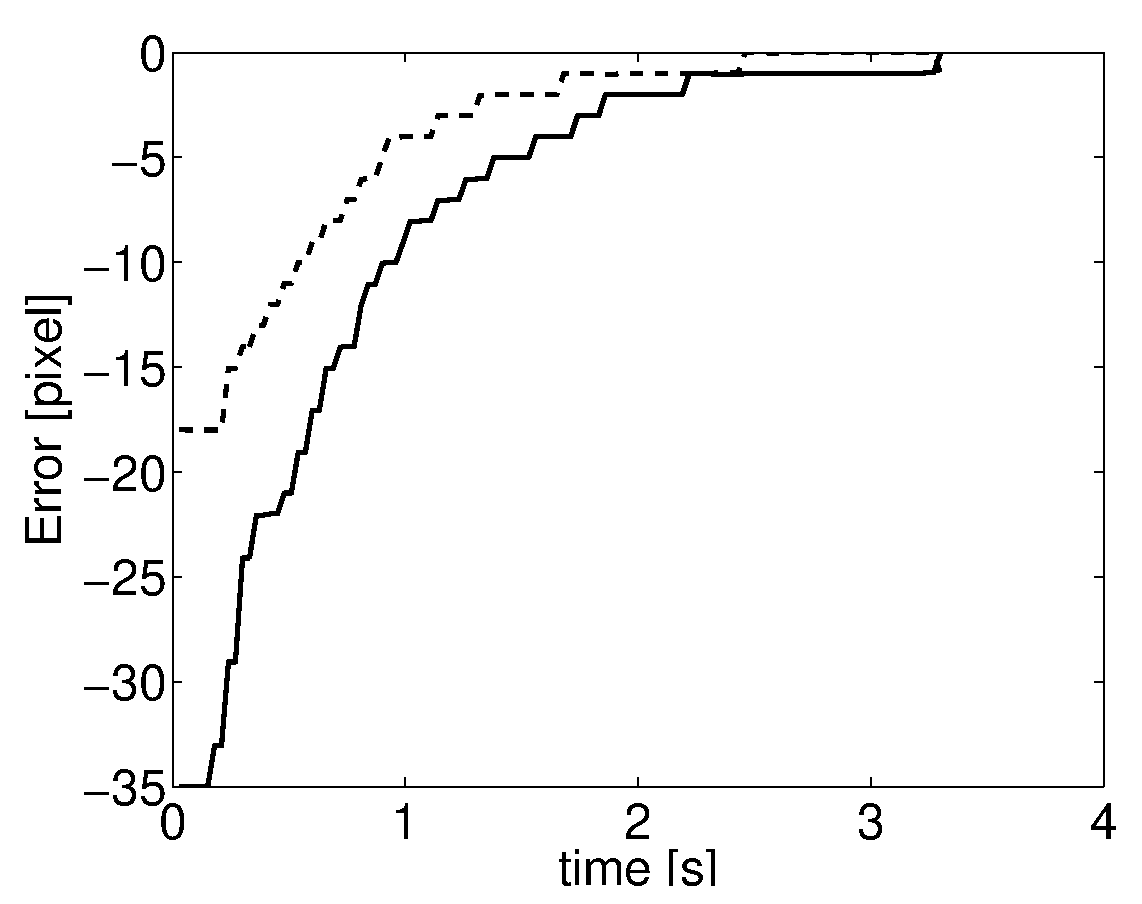
\includegraphics[width=30mm]{Figure/TimeReponseRightClosedLoop.eps}}
%	  \\
%	  \parbox{30mm}{\centering Left eye } & \hspace{0.1cm} & \parbox{30mm}{\centering Right eye }
%	  %	  \end{t\\
%	  %	Top view & & Lateral view
%  \end{tabular}
%\end{center}
%\caption{Time response of the closed loop controller. Solid lines: hand horizontal position in the left ($u_l$) and right ($u_r$). Dashed lines: vertical position, $v_l$ and $v_r$.}\label{Fig:TimeResponseClosedLoopErrors}
%  \end{figure}


\begin{figure}[th!]
  % Requires \usepackage{graphicx}
  \begin{center}
	\begin{tabular}{ccc}
	  \parbox{30mm}{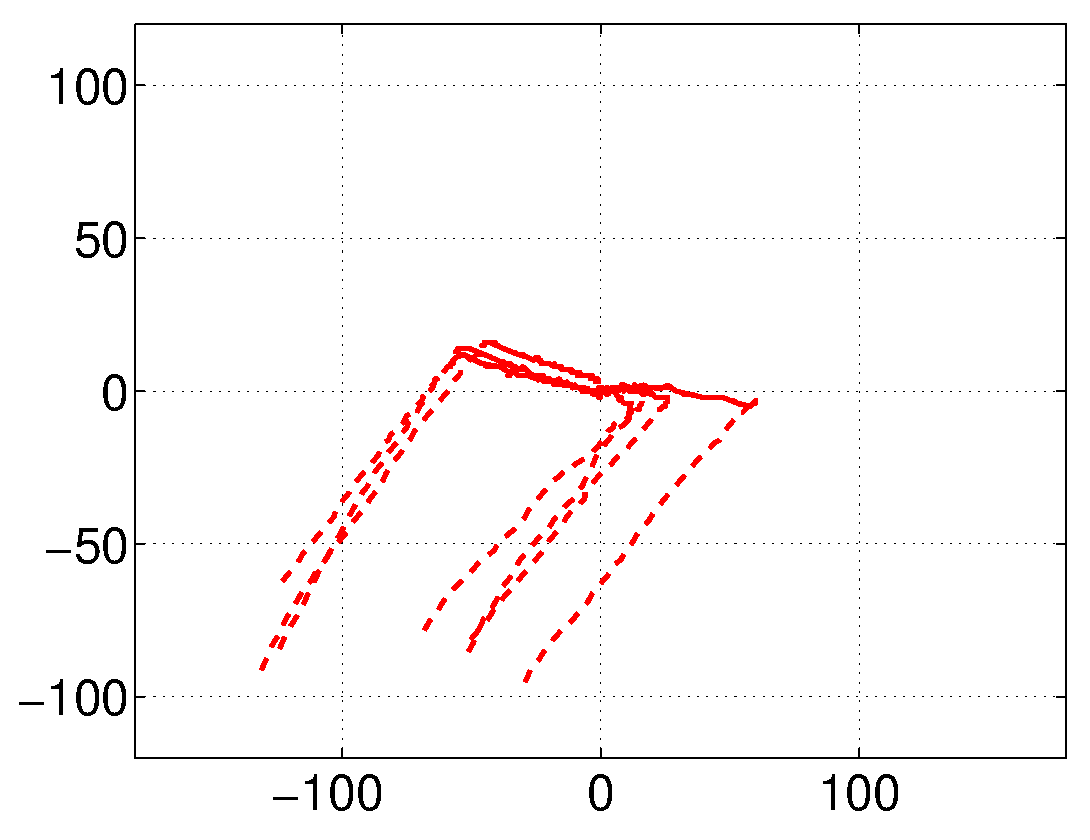
\includegraphics[width=30mm]{Figure/LeftEyeOpenClosedLoop.eps}}  & \hspace{.1cm} &
	  \parbox{30mm}{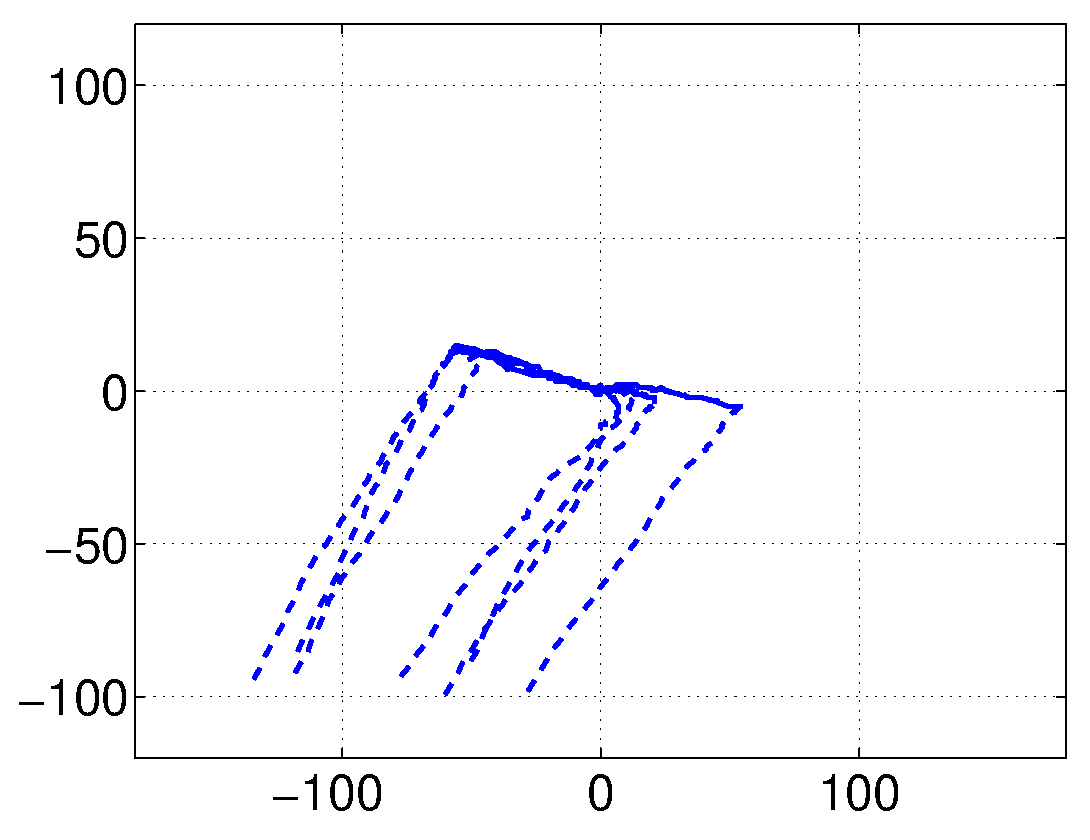
\includegraphics[width=30mm]{Figure/RightEyeOpenClosedLoop.eps}}
	  \\
	  \parbox{30mm}{\centering Left eye } & \hspace{.1cm} & \parbox{30mm}{\centering Right eye }
	  %	  \end{t\\
	  %	Top view & & Lateral view
  \end{tabular}
\end{center}
\caption{Movement of the hand on the image planes (320$\times$240)
during the execution of different reaching actions. 
Solid line: closed loop. Dashed trace: open loop. Clearly the open loop movement drives the hand to the target (the image centers) with a 
relatively small error. The closed loop phase reduces this error to zero.}\label{Fig:TimeResponseOpenClosedLoopErrors}
  \end{figure}
  
  \begin{figure}[th!]
  % Requires \usepackage{graphicx}
  \begin{center}
	\begin{tabular}{ccc}
	  \parbox{30mm}{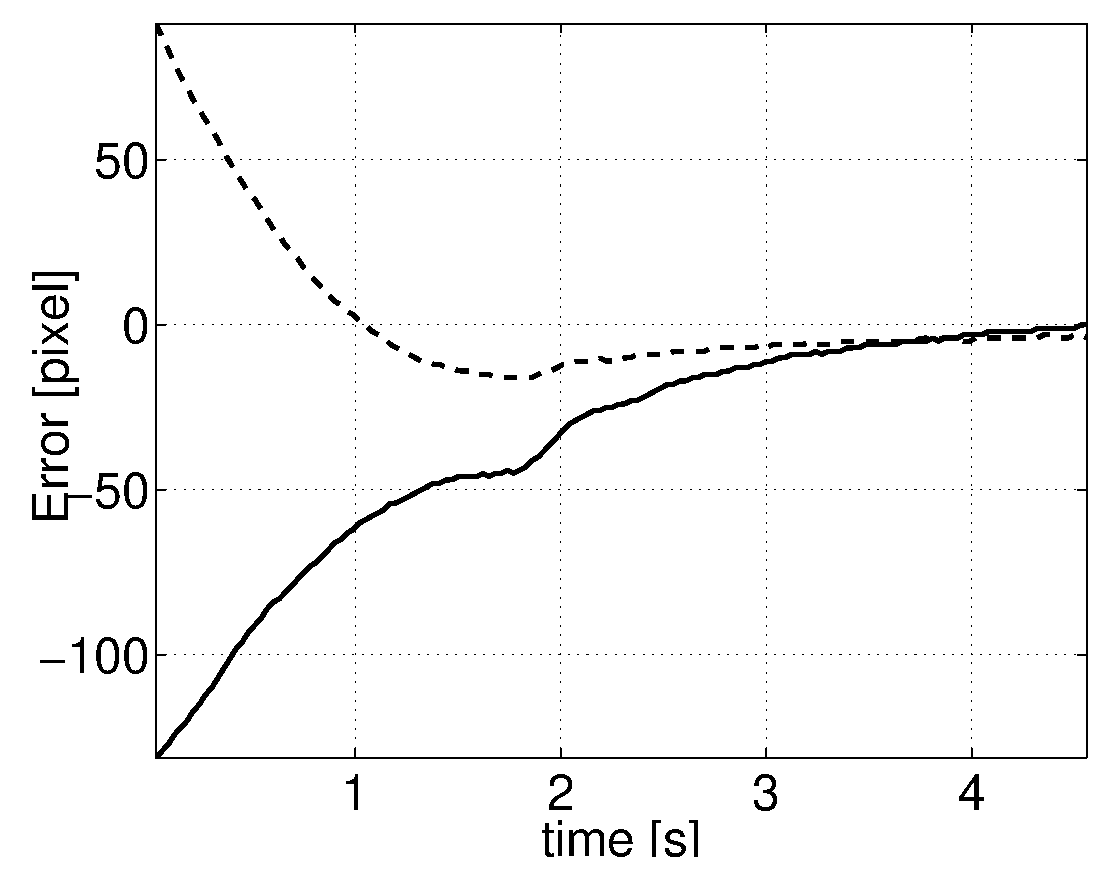
\includegraphics[width=30mm]{Figure/LeftEyeOpenClosedLoopTimeResponse.eps}}  & \hspace{.1cm} &
	  \parbox{30mm}{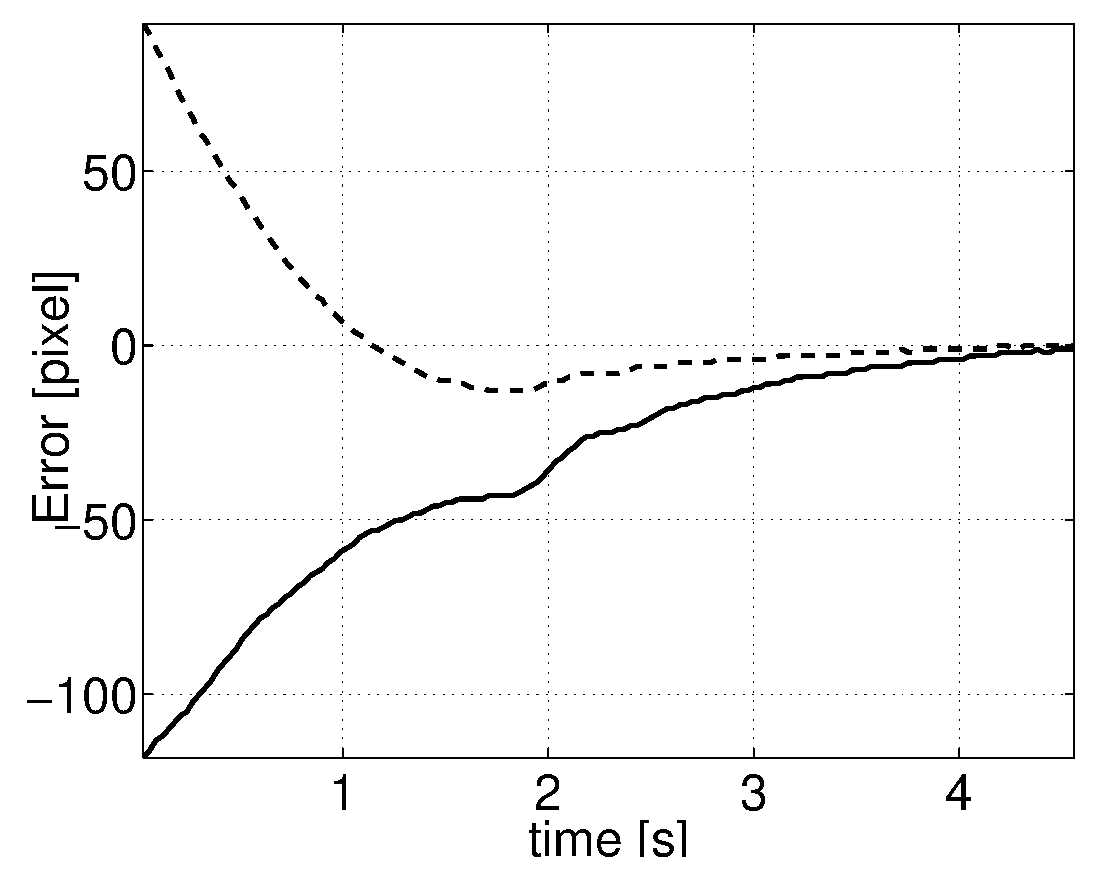
\includegraphics[width=30mm]{Figure/RightEyeOpenClosedLoopTimeResponse.eps}}
	  \\
	  \parbox{30mm}{\centering Left eye } & \hspace{.1cm} & \parbox{50mm}{\centering Right eye }
	  %	  \end{t\\
	  %	Top view & & Lateral view
  \end{tabular}
\end{center}
\caption{Time response of the closed loop and open loop strategy. Solid lines: $u_r$ and $u_l$. Dashed lines: $v_r$ and $v_l$. Remarkably, the open loop phase is faster but does not drive the hand exactly on the target. The closed loop is slower but more accurate.}\label{Fig:TimeResponseOpenClosedLoop}
\end{figure}


\subsection{Superimposed Open and Closed Loop}

Finally, we tested an alternative control strategy based on activating the closed loop 
phase immediately after the hand becomes visible on both image planes. This second strategy
is such that the open a closed loop strategies will be active at the same time for a 
certain amount of time. 
\newpage 
The structure is based on a classical control scheme, which can be represented as follows:

\begin{figure}[th!]
\begin{center}
\includegraphics[scale = 0.25]{Figure/OpenVSClosedLoop.eps}
\end{center}
\end{figure}

Practically, the feedforward control corresponds to the open loop part of the reaching movement.
It is activated exactly as described in Section \ref{sec:openReaching} and therefore it does not
require the hand to be visible in the image plane. The feedback control
instead corresponds to the closed loop part of the movement and can be activated when the hand
has been localized in both the image planes. Practically, the final solution can be described by the 
following scheme:

\begin{figure}[th!]
\begin{center}
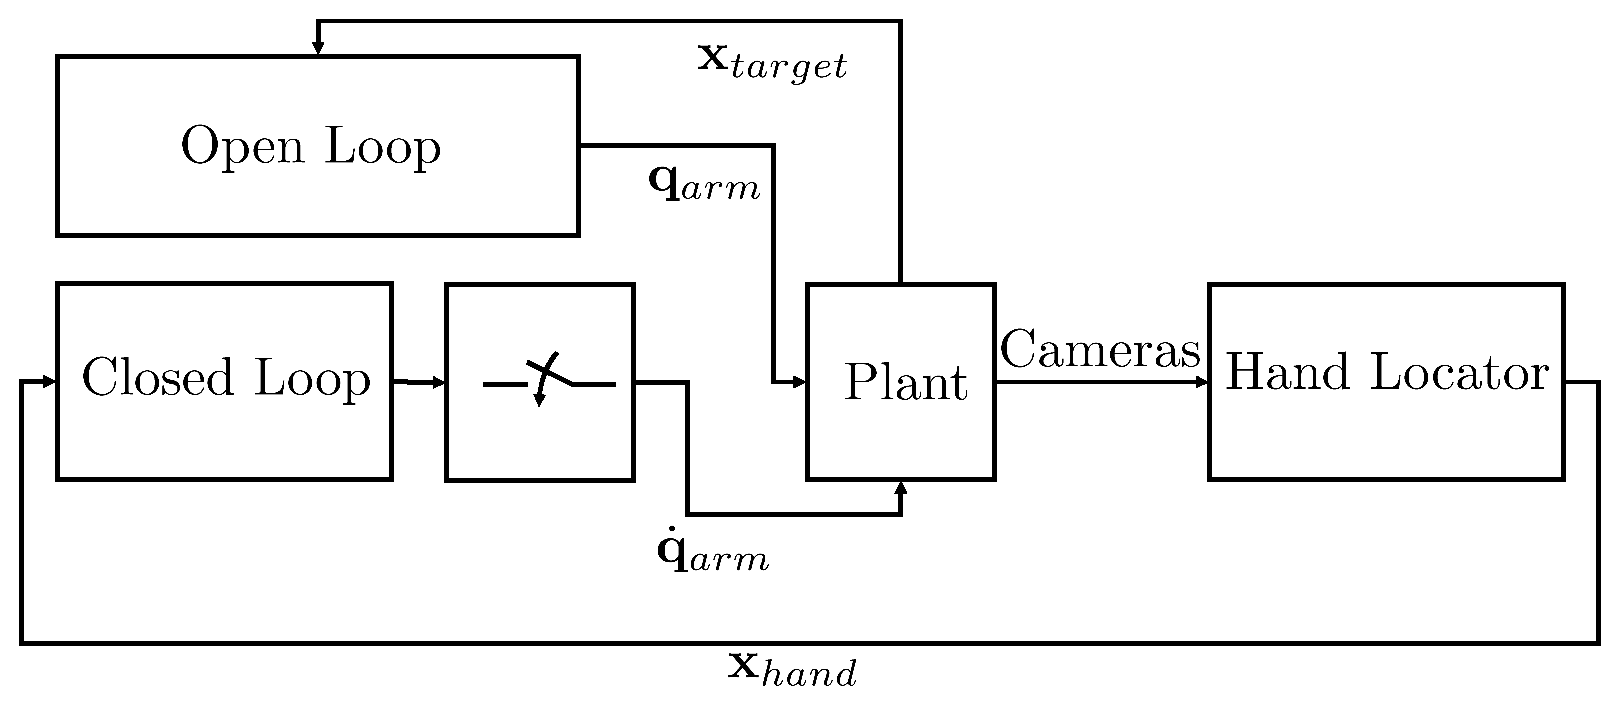
\includegraphics[scale = 0.25]{Figure/OpenVSClosedLoopSwitch.eps}
\end{center}
\end{figure}

Clearly, when both the open and closed loop controllers are active, the system receives position 
and velocity control simultaneously\footnote{A position command ${\mathbf q}_{arm,d}$ is 
always translated into a trajectory following command by moving 
the hand along a trajectory $\mathbf q_{arm}(t)$, $t \in [0, T]$ such that: $T$ is the execution time,
$\mathbf q_{arm}(0)$ is the arm position when the command is received, $\mathbf q_{arm}(T) = {\mathbf q}_{arm,d}$
is the desired final position, $\dot {\mathbf q}_{arm}(t) = 0$, $ \forall t > T$. If a velocity command $\dot {\mathbf q}_{arm,d}$ is received while executing a position
command $\mathbf q_{arm}(t)$, the original velocity command is transformed into a new one, nominally
$\dot {\mathbf q}_{arm} = \dot {\mathbf q}_{arm}(t) + \dot {\mathbf q}_{arm, d}$.}. 

A comparison between this control strategy and the one proposed in Section \ref{Eq:ClosedLoop}
is given in Figure \ref{Fig:TimeResponseOpenVSClosedLoopErrors} and \ref{Fig:TimeResponseOpenVSClosedLoop}. 
The second control strategy clearly outperforms the first one. As a matter of fact, the image plane movement (Figure \ref{Fig:TimeResponseOpenVSClosedLoopErrors})
is much more regular resulting in a unique linear movement instead of begin divided into two segments. Secondly, the
execution time is clearly reduced as it can be noted in Figure \ref{Fig:TimeResponseOpenVSClosedLoop}.


\begin{figure}
  % Requires \usepackage{graphicx}
  \begin{center}
	\begin{tabular}{ccc}
	  \parbox{30mm}{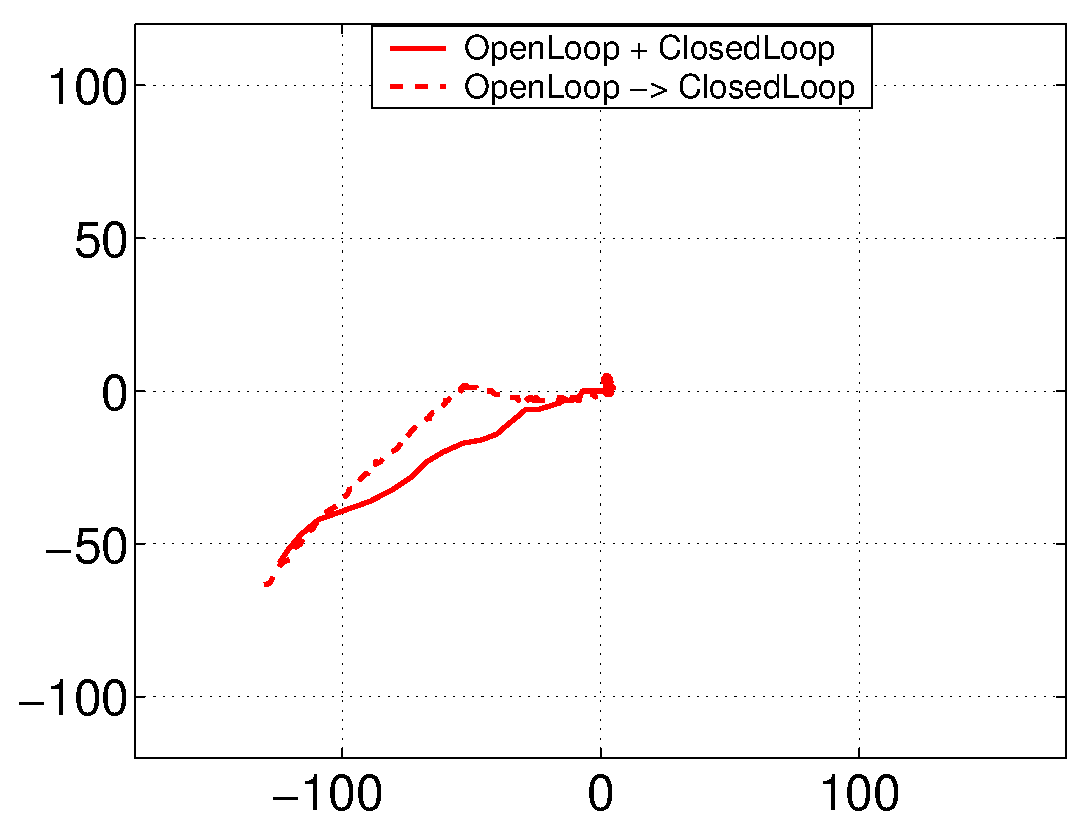
\includegraphics[width=30mm]{Figure/LeftEyeOpenVSClosedLoop.eps}}  & \hspace{.1cm} &
	  \parbox{30mm}{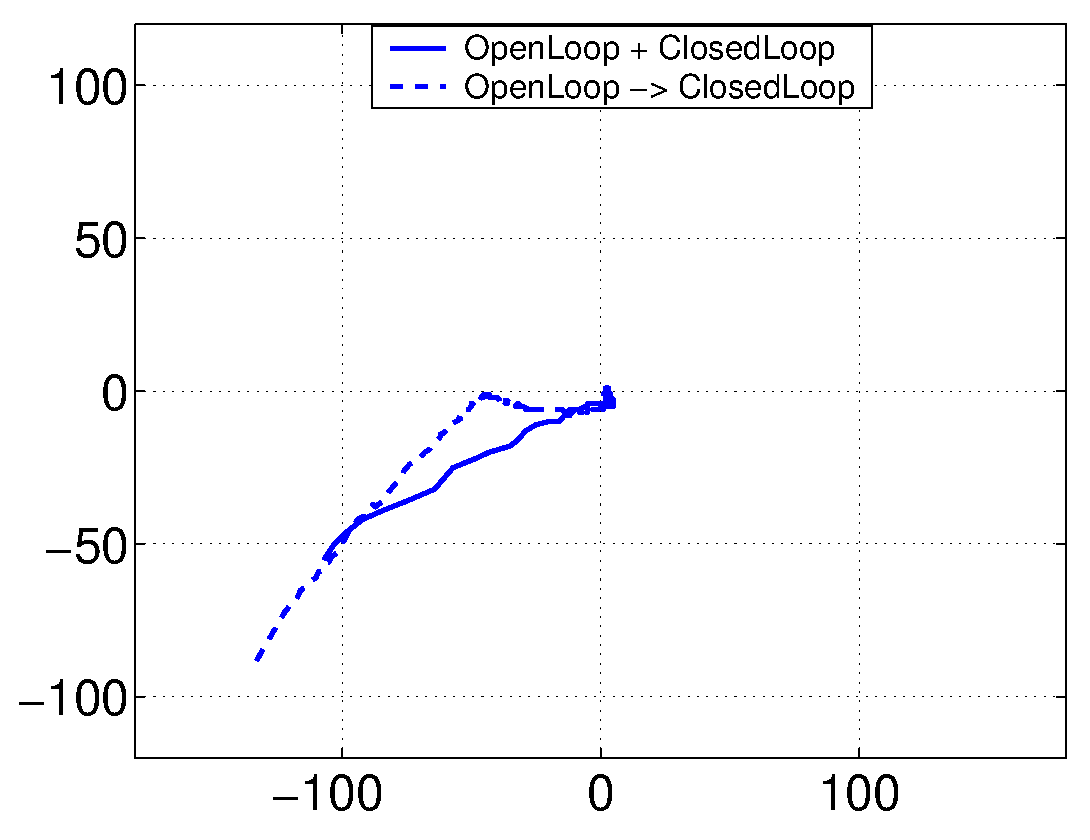
\includegraphics[width=30mm]{Figure/RightEyeOpenVSClosedLoop.eps}}
	  \\
	  \parbox{30mm}{\centering Left eye } & \hspace{.1cm} & \parbox{30mm}{\centering Right eye }
	  %	  \end{t\\
	  %	Top view & & Lateral view
  \end{tabular}
\end{center}
\caption{Movement of the hand on the image planes ($320 \times 240$)
during the execution of a single reaching movement. Dashed line: hand movement
during an open loop movement followed by a closed loop phase. Solid line: hand movement during 
the superposition of open and closed loop strategies.}\label{Fig:TimeResponseOpenVSClosedLoopErrors}
  \end{figure}
  
  \begin{figure}
  % Requires \usepackage{graphicx}
  \begin{center}
	  \parbox{40mm}{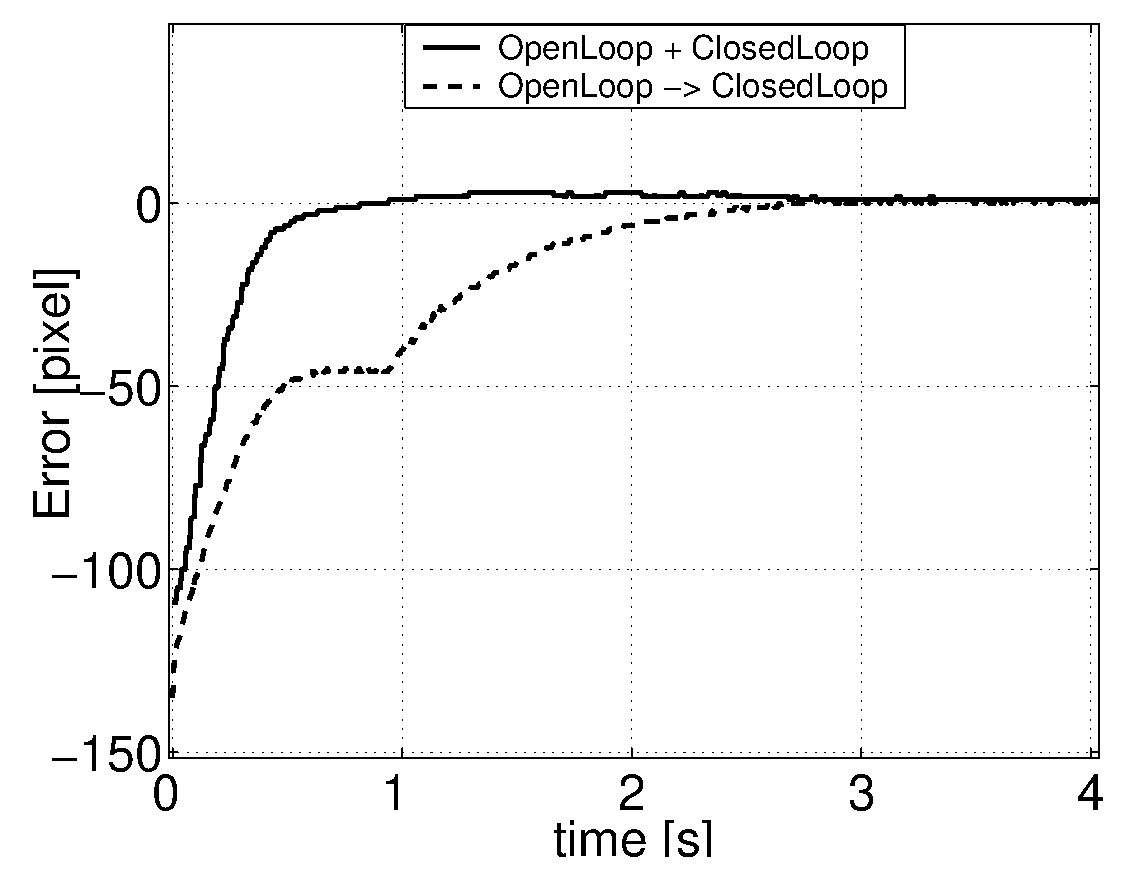
\includegraphics[width=40mm]{Figure/OpenVSClosedLoopTimeResponse1.eps}}
  \end{center}
\caption{Time response of the image plane position $u_l$. Dashed line: hand movement
during an open loop movement followed by a closed loop phase. Solid line: superposition of open and closed loop strategies.
 Remarkably, this second control architecture results in a faster response because when the hand becomes visible it is 
directly driven to the target without waiting for the open loop phase end.}\label{Fig:TimeResponseOpenVSClosedLoop}
  \end{figure}

\subsection{Null space movement}

In order to validate the quality of the Jacobian estimation, we tested the effects of a null space movement 
on the primary task (keeping $\uhand = 0$) as proposed in \cite{Mansard06jacobian}. A simple way to perform this testing is the following control strategy:
\begin{equation} \label{Eq:ClosedLoopStrategyRedundant}
\mathbf{\dot q}_{arm}=-k_1 \cdot \jacobian^\# \uhand + k_2 (I - \jacobian^\# \jacobian) \mathbf w, 
\end{equation}
where $I \in \mathbb R^{4 \times 4}$ is the identity matrix, $\mathbf w \neq 0$ is a 
randomly chosen vector in $\mathbb R^4$ and $k_1$, $k_2$ are positive constants. 
Ideally, the strategy (\ref{Eq:ClosedLoopStrategyRedundant}) should allow arm movements 
$\mathbf{q}_{arm} \neq 0$ while leaving the hand position $\uhand$ unperturbed. Practically we observed 
a minimal image plane movement (Figure \ref{Fig:RedundancyImagePlane})
as oppposed to a relatively large arm movement (Figure \ref{Fig:RedundancyArm}). These results 
further prove the quality of our Jacobian estimation.

\begin{figure}
  % Requires \usepackage{graphicx}
  \begin{center}
	\begin{tabular}{ccc}
	  \parbox{30mm}{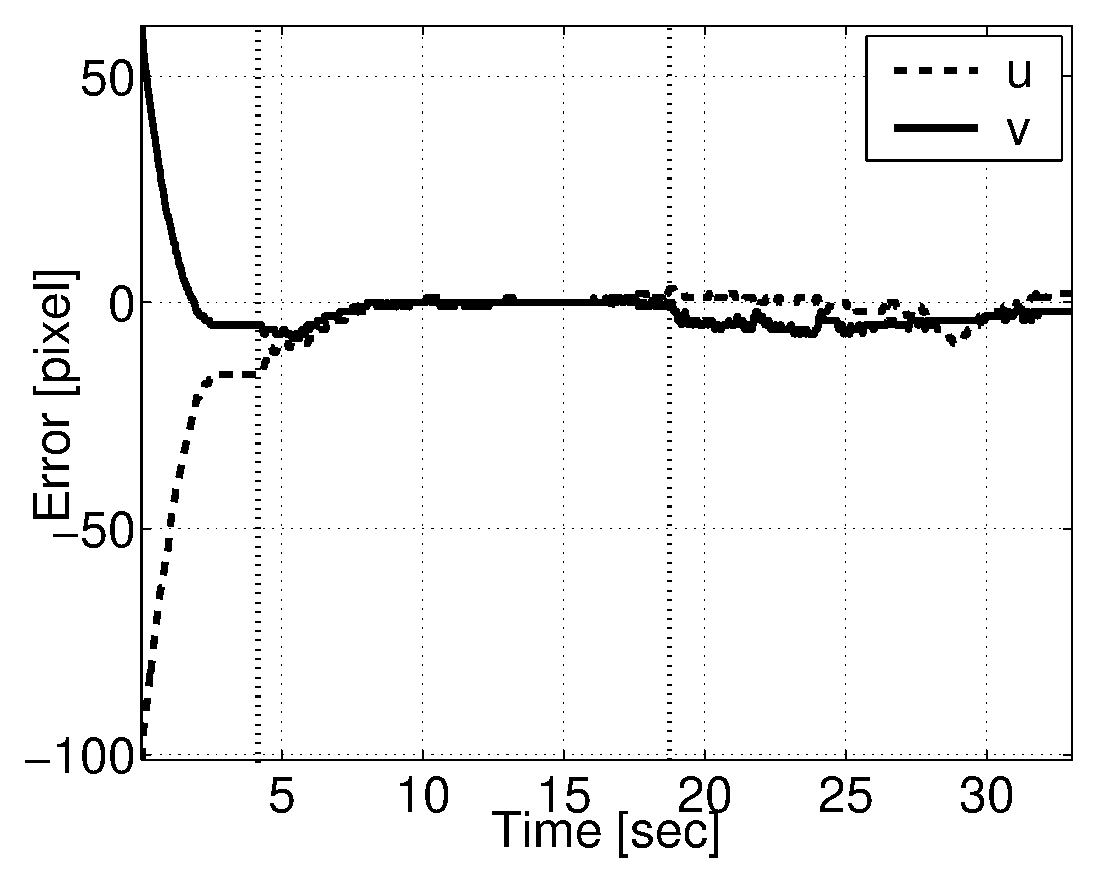
\includegraphics[width=30mm]{Figure/RedundancyLeft.eps}}  & \hspace{.1cm} &
	  \parbox{30mm}{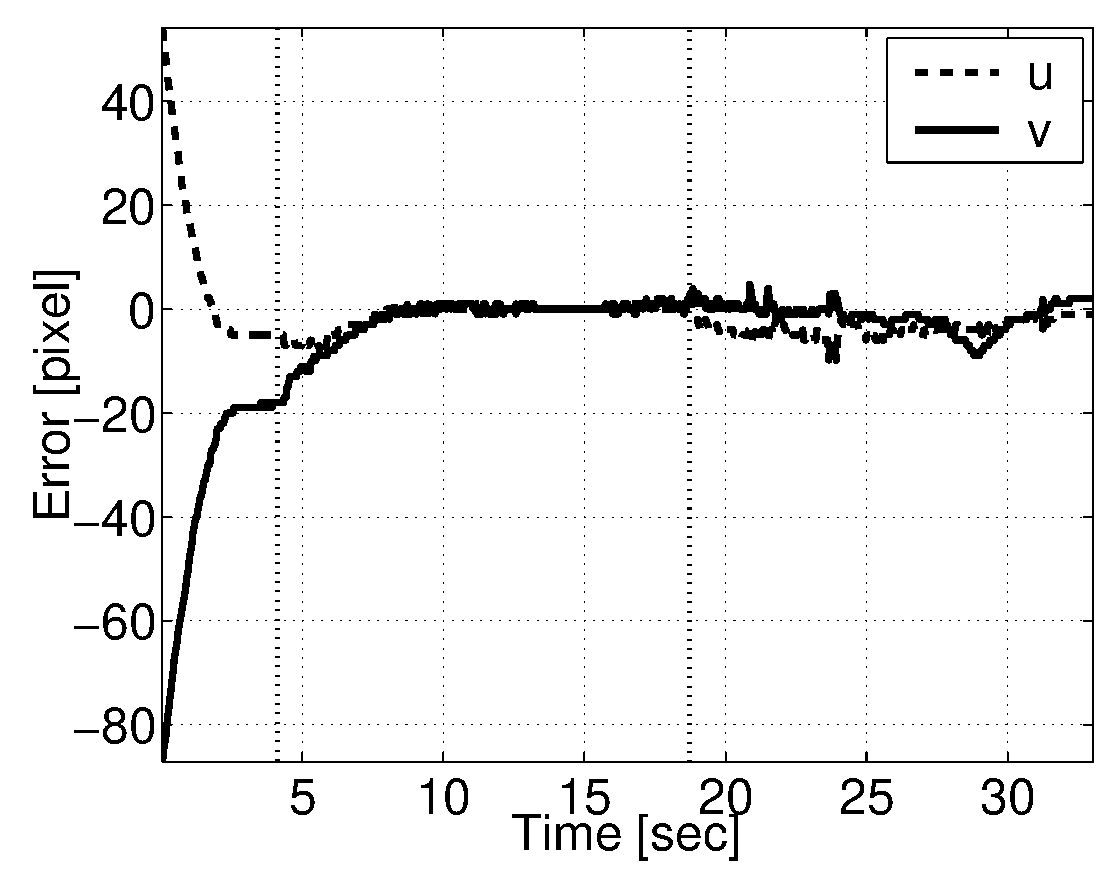
\includegraphics[width=30mm]{Figure/RedundancyRight.eps}}
	  \\
	  \parbox{30mm}{\centering Left eye } & \hspace{.1cm} & \parbox{30mm}{\centering Right eye }
	  %	  \end{t\\
	  %	Top view & & Lateral view
  \end{tabular}
\end{center}
\caption{Image plane movements during a three phase reaching. 
First the open loop, then the closed loop and finally a movement 
in the null space of the given task (keeping the hand in fixations). 
Each phase is delimited by a vertical dotted line.
}\label{Fig:RedundancyImagePlane}
  \end{figure}
  
  \begin{figure}
  % Requires \usepackage{graphicx}
  \begin{center}
	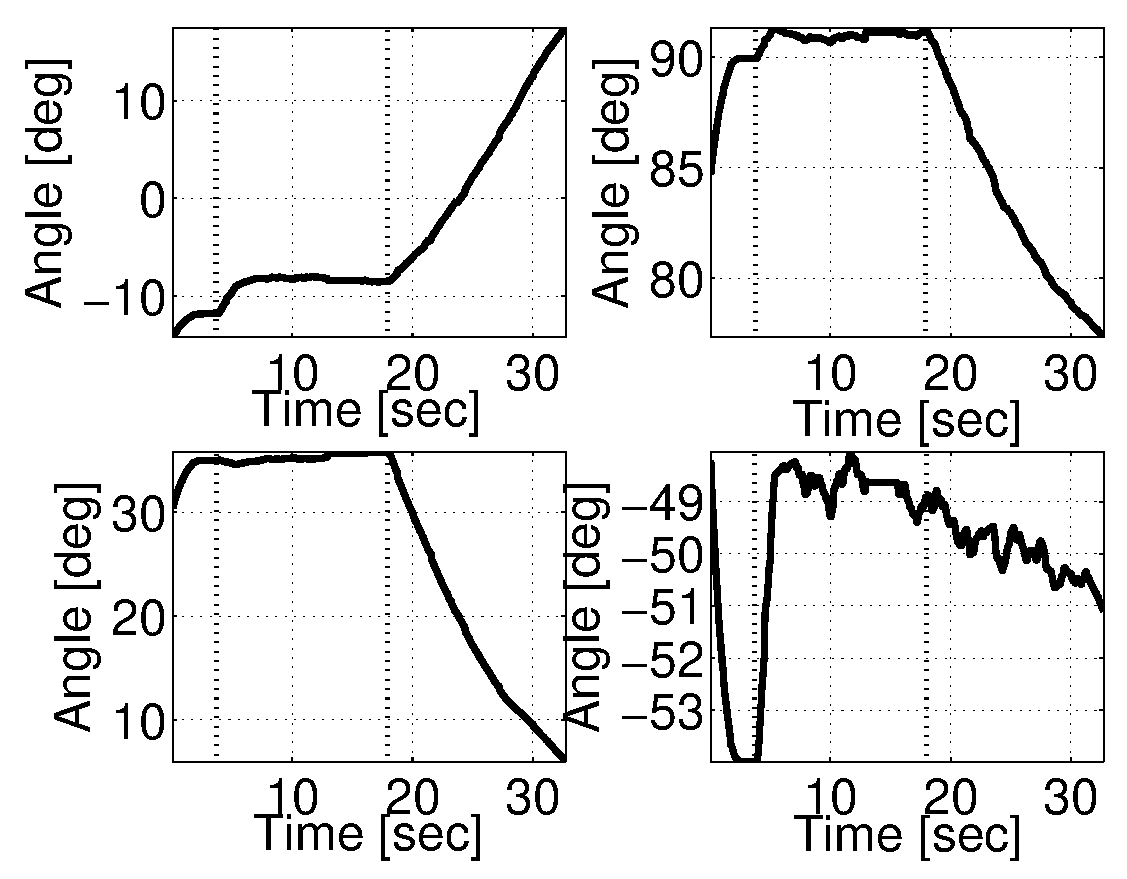
\includegraphics[width=60mm]{Figure/RedundancyArm.eps}
	\end{center}
\caption{Arm movement corresponding to the image plane movements shown in Figure \ref{Fig:RedundancyImagePlane}.
 Remarkably, the null space movement is characterized by large joint movements which are however not visible 
in the image plane due to the jacobian based compensation.} \label{Fig:RedundancyArm}
  \end{figure}
\section{Conclusions}
In this paper we have described the implementation of a reaching
behavior that integrates together an open loop and a closed 
loop controller. The open loop controller
allows the robot to perform faster movements and does not require visual 
feedback from the hand. When sight of the hand is available the closed
loop controller allows for precise positioning of the hand in the 
image plane. 

We describe an explorative strategy by which the robot autonomously 
acquires the forward motor map and the visual Jacobian transformations. 
Among the other things this strategy 
allows the estimation of the eye-to-hand visual Jacobian of the robot. 
The estimation of the Jacobian is a well studied task for which several 
solutions have been proposed \cite{Hosoda94versatile,Mansard06jacobian,
Lapreste04efficient}. None of these works, however, addresses the 
problem of the redundancy of both the head and the arm. In the experiments 
reported here the estimation of the Jacobian is performed with good 
accuracy for a subset of the arm workspace and for 
\emph{different head postures}. We believe
this is an important contribution with respect to the state of the art.

We do not rely on any prior information about the 
kinematic structure of the robot. The only simplification was that we used 
a color marker to visually localize the hand of the robot. Our assumption
is that the hand localization/identification is a separate problem
that needs to be solved before learning reaching. Previous work
by the same and other authors have suggested procedures by which 
the robot could autonomously learn to solve this task 
(\cite{Natale05,edsinger06what}). It will be interesting to see
how these approaches can be integrated with the work described 
in this paper.

\section*{Acknowledgement}
% optional entry into table of contents (if used)
%\addcontentsline{toc}{section}{Acknowledgment}
The work presented in this paper
has been supported by the \textsc{RobotCub} project (IST-2004-004370), funded by the
European Commission through the Unit E5 ``Cognitive Systems''. Moreover, it has
been partially supported by \textsc{Neurobotics}, a European FP6 
project (IST-2003-511492) and \textsc{Contact} (NEST 5010).




%

% references section
%%% this must be IEEEtran
\bibliographystyle{IEEEtran}
\bibliography{main}

\end{document}




